\documentclass[11pt,twosided]{article}
\usepackage{amsmath,amsfonts,amsthm,amssymb}
\usepackage{amstext}
\usepackage{setspace}
\usepackage{Tabbing}
\usepackage{fancyhdr}
\usepackage{lastpage}
\usepackage{extramarks}
\usepackage{chngpage}
\usepackage{soul,color}
\usepackage[pdftex]{graphicx}
\usepackage{longtable}
\usepackage{hyperref}
%\usepackage{minitoc}
\usepackage{authblk}
\usepackage{enumerate}
\usepackage{listings}
\usepackage[round]{natbib}
%\usepackage[square]{natbib}
\usepackage{fancyvrb}
\usepackage[most]{tcolorbox}
\DefineVerbatimEnvironment{code}{Verbatim}{fontsize=\small}
\DefineVerbatimEnvironment{example}{Verbatim}{fontsize=\small}
\urlstyle{same}
\usepackage{url}
\usepackage{menukeys}
\usepackage{tabularx}
\usepackage{booktabs}

%\setlength{\parskip}{0pt}
%\setlength{\parsep}{0pt}
%\setlength{\headsep}{0pt}
%\setlength{\topskip}{0pt}
%\setlength{\topmargin}{0pt}
%\setlength{\topsep}{0pt}
%\setlength{\partopsep}{0pt}
%\linespread{0.75}

%\lhead{V. CHHATRE}
\lhead{Sheridan Workshop}
\chead{}
\rhead{R Data Visualization}
%\rhead{}
\lfoot{}
\cfoot{}
\cfoot{\thepage}
\rfoot{}
%\renewcommand\headrulewidth{0.4pt}
%\renewcommand\footrulewidth{0.4pt}

\title{
\includegraphics[width=1in]{uwlogo}\\
\vspace{1in}  
{\huge INBRE Bioinformatics Core \\\vspace{5pt} {\LARGE WYCC Workshop Series}} \\
\begin{center}
\rule{6in}{0.4pt}\\\vspace{0.2in}
{\huge Data Analysis \& Visualization in R \\\vspace{0.15in} {\LARGE Phenological Onset of Spring}}\\
\vspace{0.15in}
\rule{6in}{0.4pt}\\
\end{center}
\vspace{1in}
}


\author{{\LARGE Vikram E. Chhatre \\ University of Wyoming} \\
\vspace{2ex}
{\large \href{mailto:vchhatre@uwyo.edu}{vchhatre@uwyo.edu} \\
}}

\date{April 4, 2017}



% In case you need to adjust margins:
\topmargin=-0.55in      %
\evensidemargin=0in     %
\oddsidemargin=0in      %
\textwidth=6.5in        %
\textheight=8.8in       %
%\headsep=0.15in         %


\begin{document}
\pagestyle{fancy}
\maketitle

\thispagestyle{empty}

\clearpage
\tableofcontents
\clearpage
\parindent=0em


\section{Working with R}
R (\url{http://www.r-project.org}) is an open source, statistical data analysis and visualization language. Our goals today are: (1) to become familiar with the basic functionality included in R, (2) perform some statistical data analysis, (3) prepare plots/graphs that depict information in visual form and finally, (4) to use a specific R package (packages are explained in section 3.1) called {\tt ggplot2} to visually display `Onset of Spring' data across 48 US states.\\

\subsection{Launch RStudio}
R can run both within the terminal shell or as a standalone GUI application (e.g. RStudio).  You will be using RStudio.  Regardless of what method you use to launch R, the output is the same.  Launch a new R session with RStudio by double clicking its icon.  RStudio is just the wrapper graphical user interface for the underlying programming langugage R:\\

%\begin{tcolorbox}[boxrule=0.5pt]
%\begin{code}
%[train@localhost ~]$ cd /home/train/
%[train@localhost ~]$ R
%
%R version 3.3.1 (2016-06-21) -- "Bug in Your Hair"
%Copyright (C) 2016 The R Foundation for Statistical Computing
%Platform: x86_64-apple-darwin13.4.0 (64-bit)
%
%>
%\end{code}
%\end{tcolorbox}
%\vspace{2ex}

\begin{center}
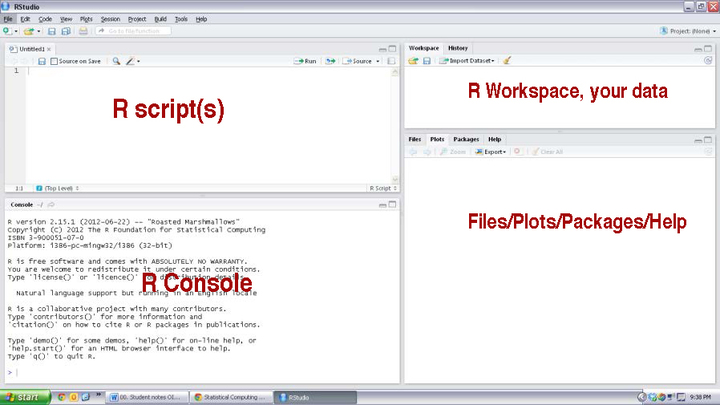
\includegraphics[width=7in]{rstudio}
\end{center}

\subsection{RStudio Panel Components}
\begin{itemize}
\item {R Script:} This is the area where you write commands, programs, etc. You can run single lines of
code or code blocks using keyboard shortcuts or buttons in the header. The entire script can be
saved as a filename.R file, allowing you to use it again later.


\item {\bf Console:} This is where the commands from your Script are actually executed. Nothing here is
saved. You can type individual commands here, but you can’t recapture what you have done as a
script. Commands are executed when you choose ENTER. The up arrow on the keyboard can be
used to select and repeat earlier commands in the console. Similar to how the Terminal operates.

\item {\bf Workspace:} This is where objects created by your script are temporarily stored. These objects are
lost when you exit the program. It can be useful to view you objects and review variable names and
types in this window.

\item {\bf Files/Plots/Packages/Help:} Plots are where graphics are displayed. You can use the arrow to
cycle between your graphs. None of these are saved unless you export them. You can export images
as PDFs from here or add code to your script to save images as svg, png, etc. Packages shows
packages you have download and installed to your base R program. If you need to add a package,
you can Google the one you want, download it, and choose “Install packages” from the Packages
menu. The packages will be saved on your computer, but will have to be called in your code each
time you need them. Help provides access to information about commands.
\end{itemize}


Today, you will be typing all of the commands inside the {\bf Console} window.  You know R is expecting an input from you when it presents you with the {\tt >} prompt.  Every time you type a command at the prompt, R performs that task and then brings you back to the prompt on the next line.  In other words, this prompt is your visual cue that R is ready to take another command from you.

\subsection{R as Calculator}
In one of its simplest incarnations, R can be used a calculator.  Try the following exercises.  No matter how difficult the calculations, R will return instantaneous results.  You will also find that R will also solve rather long and complex calculations, which are tedious to perform on a graphical calculator.\\

\begin{tcolorbox}[boxrule=0.5pt]
\begin{code}
> 2223482 + 98979723

> 55/279

> 1e-3

> 10^-20

> 4.58*2000

\end{code}
\end{tcolorbox}
\vspace{2ex}

\subsection{Data Analysis using R}

Before you can analyze it, you need to load data in R.  This can be accomplished in a multitude of ways.  You can even create data on the fly.  The following example demonstrates preparing a simple datum from within R.  

\subsubsection{Your First Data Set}
First we create a vector called {\tt tempC} which contains a list of temperatures in degrees centigrade.  Each temperature is separated from the next by a comma.  If you now type {\tt tempC} at the R prompt, it will print all those temperature values.  Congratulations, you just crated a new datum on the fly.\\

\begin{tcolorbox}[boxrule=0.5pt]
\begin{code}
> tempC <- c(-50, -38, -22, -5, 0, 5, 8, 11, 25, 30, 36)
> tempC
[1] -50 -38 -22  -5   0   5   8  11  25  30  36
\end{code}
\end{tcolorbox}
\vspace{2ex}

Note that the variable {\tt tempC} is now stored in R's memory and you can also graphically display it in the upper-right hand pane of the RStudio window.  Next, let's create another datum using the first datum and the calculator function built into R. We will convert the vector {\tt tempC} into another vector named {\tt tempF}, which will contain respective temperatures in degrees Fahrenheit.\\

\begin{tcolorbox}[boxrule=0.5pt]
\begin{code}
> tempF <- tempC * 1.8 + 32
> tempF
[1] -58.0 -36.4  -7.6  23.0  32.0  41.0  46.4  51.8  77.0  86.0  96.8
\end{code}
\end{tcolorbox}
\vspace{2ex}


\subsubsection{Your First R Plot}
Does this example make you curious about the relationship between the two metrics of temperature measurement?  If so, we can visualize this relationship quickly using a simple plotting function.  At its simplest, a plot requires only two things: the {\tt x} and the {\tt y} values.  Let's plot our two vectors as follows:\\

\begin{tcolorbox}[boxrule=0.5pt]
\begin{code}
> plot(tempC, tempF) 
\end{code}
\end{tcolorbox}
\vspace{2ex}

This is a bare minimum plot and it conveys all necessary information.  But you can also control many aesthetic features of this plot using subfunctions within the {\tt plot()} command.  Let's try out some examples.  Each successive example command builds upon the previous one and the final command combines all intermediate steps into one:\\

\begin{tcolorbox}[breakable,boxrule=0.5pt,enhanced]
\begin{code}
> plot(tempC, tempF, xlab=`Temp (C)') 
> plot(tempC, tempF, xlab=`Temp (C)', ylab=`Temp (F)') 
> plot(tempC, tempF, xlab=`Temp (C)', ylab=`Temp (F)', pch=16) 
> plot(tempC, tempF, xlab=`Temp (C)', ylab=`Temp (F)', pch=16, col=`salmon') 
> plot(tempC, tempF, xlab=`Temp (C)', ylab=`Temp (F)', pch=16, col=`salmon', 
  main=`Relationship between C and F') 
> abline(lm(tempF~tempC), col=`black')
\end{code}
\end{tcolorbox}
\vspace{2ex}

What is the last line of code doing?  It's basically plotting a {\bf best fit} line using linear regression method.  You will need the last two lines of code to get the complete plot.  The last line does not work by itself.  It must come immediately after the {\tt plot()} command.  You may be wondering, `what if I want to save this plot into a file?'.  R allows you save plots into various types of file formats, such as {\tt .pdf}, {\tt .png}, {\tt .jpg}, {\tt .tif} and also scalable vector graphics format i.e. {\tt .svg}.  You just need to wrap the above two lines of code inside an open device (format) and then close the device.  See the example below:\\


\begin{tcolorbox}[breakable,boxrule=0.5pt,enhanced]
\begin{code}
> pdf(`tempC_vs_tempF.pdf')
> plot(tempC, tempF, xlab=`Temp (C)', ylab=`Temp (F)', pch=16, col=`salmon', 
  main=`Relationship between C and F')
> abline(lm(tempF~tempC), col=`black')
> dev.off()
\end{code}
\end{tcolorbox}
\vspace{2ex}

That's it.  You have now successfully created a pdf file containing the above plot.\\


\subsubsection{A Second Example}
Let's do a bit more advanced example now with your newfound knowledge.  Every R distribution comes with various example data sets already prepared.  We will use one such data set called {\tt co2}, which contains data on carbon dioxide levels (in ppm) recorded since 1959 at Hawaii's Manoa Loa Research Station. It's a monthly time series of carbon dioxide levels starting in year 1959 and ending in year 1997. \\


\begin{tcolorbox}[breakable,boxrule=0.5pt,enhanced]
\begin{code}
> data(co2)
> head(co2)
[1] 315.42 316.31 316.50 317.56 318.13 318.00
\end{code}
\end{tcolorbox}
\vspace{2ex}

The {\tt head} command allows you to look at the first few lines of a given data set.  So why are we seeing only a few numbers here?  That's because this data is a time series.  How can you know if a given data is time series?  R provides a function for checking the {\tt class} of the data.  For a time series, one should also check the size of this time series.  See the example below:\\

\begin{tcolorbox}[breakable,boxrule=0.5pt,enhanced]
\begin{code}
> class(co2)
"ts"

> length(co2)
468
\end{code}
\end{tcolorbox}
\vspace{2ex}

As you can see, R lists the class of this data set as {\tt ts} or time series.  The length of the data set is 468, that is 12 observations per month for 39 consecutive years.  For timeseries, plotting is extremely easy.  See below.  Notice that we did not use x and y variables here since the data is not two dimensional.  Merely providing name of the dataset is sufficient for R to draw a plot.  Do you remember how to save this plot into a {\tt pdf} file?  Try saving it as a {\tt png} image this time instead.\\

\begin{tcolorbox}[breakable,boxrule=0.5pt,enhanced]
\begin{code}
> plot(co2)
\end{code}
\end{tcolorbox}
\vspace{2ex}

The aesthetics of the plot can be enhanced as in the previous example.  Try the following code:\\

\begin{tcolorbox}[breakable,boxrule=0.5pt,enhanced]
\begin{code}
> pdf(`co2_conc_HI.pdf')
> plot(co2, col=`orange', lwd=1.5, main=`Atmospheric CO2 (ppm) at Manoa Loa, Hawaii')
> dev.off()
\end{code}
\end{tcolorbox}


\begin{center}
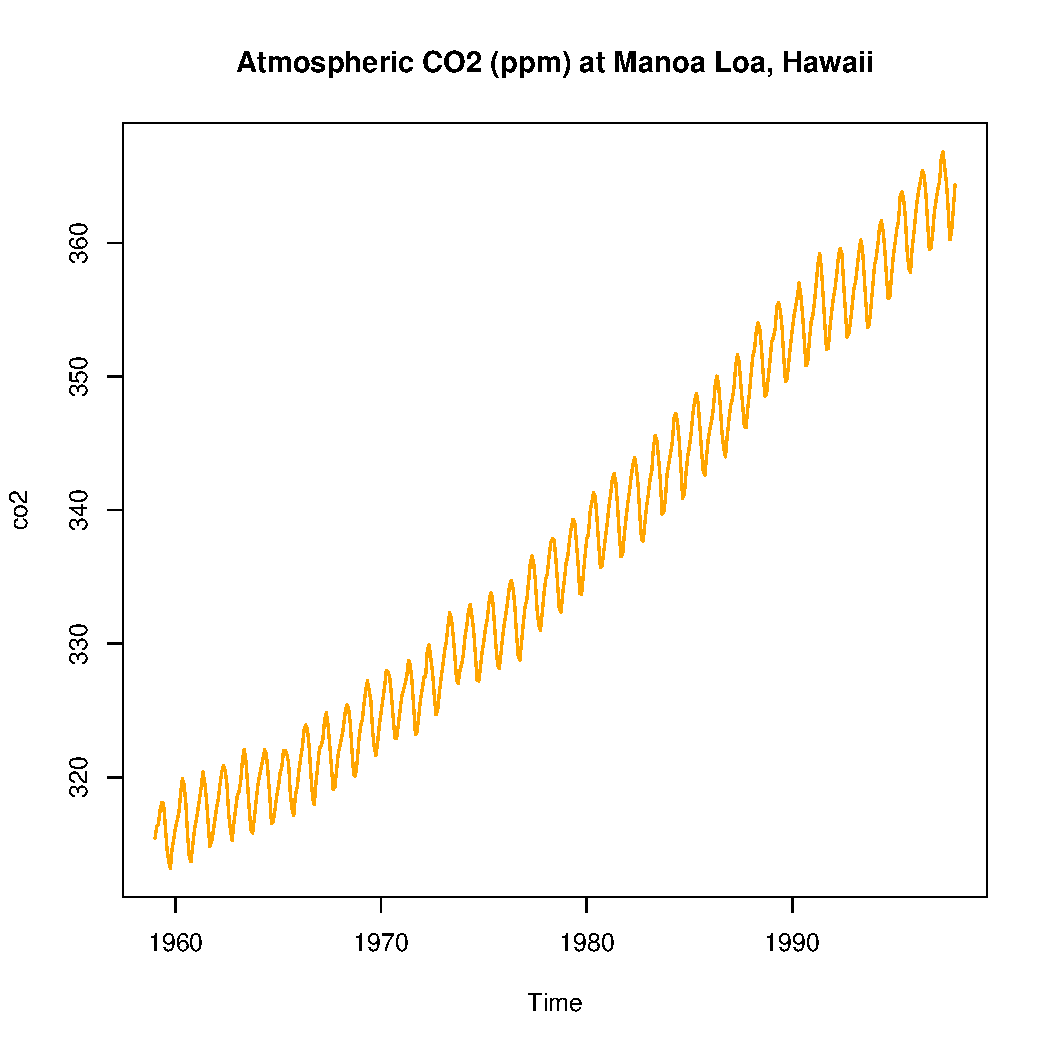
\includegraphics[width=6in]{co2_conc_HI}
\end{center}

One nice feature of RStudio is that it keeps all the plots you generate in memory.  You can flip through them (both forwards and backwards) inside the Plot pane of RStudio.  Try it out now that you have generated a couple of plots.\\

R also allows you to quickly calculate summary statistics such as mean, median, max etc. on any data set with just one command.  Likewise, you can also calculate quantiles for a variable.  \\

\begin{tcolorbox}[breakable,boxrule=0.5pt,enhanced]
\begin{code}
> summary(co2)
   Min. 1st Qu.  Median    Mean 3rd Qu.    Max. 
  313.2   323.5   335.2   337.1   350.3   366.8 

> quantile(co2)
     0%     25%     50%     75%    100% 
313.180 323.530 335.170 350.255 366.840 
\end{code}
\end{tcolorbox}

\newpage
\section{Phenological Onset of Spring}

Now that you are equipped with some working knowledge of R, we will move on to a much more interesting data set.  As explained during the lecture, National Phenology Network is an organization that keeps track of how plants exhibit different traits through seasons.  This plant activity through seasons is termed as {\bf phenology}.  Temperature and photoperiod are both important determinants of growth in plants, which are tied to geography (latitude, longitude and elevation).  Changing climate is affecting the plant phenological responses and the NPN data allows us to understand this better.\\

An important determinant of the onset of growing season in plants is the breaking of dormant buds and emergence of leaves. These buds would have been formed at the end of the previous year's growing season.  The buds overwinter and the plants have molecular genetic mechanisms to keep track of heat sums.  Once these heat sums cross a certain threshold, plants begin the process of releasing the dormancy and breaking the buds to develop new leaves.

\subsection{The Dataset}
The data we will be using today has been collected for 110 broad leaved and deciduous tree genera across the 48 contiguous US states.  Before we could look at this data, we first need to load it into R.  Unlike our previous examples, this data set is not already embedded into R.  So we will need to manually import it as follows:\\

     
\begin{tcolorbox}[breakable,boxrule=0.5pt,enhanced]
\begin{code}
> pheno <- read.csv(`pheno.csv', header=T, sep=`,')
\end{code}
\end{tcolorbox}
\vspace{2ex}

If R returned with a new prompt and no error message, the data file was read correctly. Let's get to know this data first by interacting with it.\\


     
\begin{tcolorbox}[breakable,boxrule=0.5pt,enhanced]
\begin{code}
> dim(pheno)
26869	14

> class(pheno)
"data.frame"
\end{code}
\end{tcolorbox}
\vspace{2ex}

There are 26731 rows and 14 columns in this data file. R is treating it as a {\tt data frame}.  You could use the command {\tt head} to check the first few rows of this data.  But before you do that, let's check the names of columns to get an idea.\\

     
\begin{tcolorbox}[breakable,boxrule=0.5pt,enhanced]
\begin{code}
> names(pheno)
 [1] "Site_Name"              "Latitude"               "Longitude"             
 [4] "Elevation_in_Meters"    "State"                  "Genus"                 
 [7] "Species"                "Phenophase_Description" "Mean_First_Yes_Year"   
[10] "Median_First_Yes_DOY"   "Mean_AGDD"              "Mean_Daylength"        
[13] "Tmax_Spring"            "Prcp_Spring"           
\end{code}
\end{tcolorbox}
\vspace{2ex}

Here is a brief description of the data present in each column of this data frame.\\

\begin{table}[!h]
\begin{tabular}{l p{4.5in}}
\toprule\\[1ex]
{\bf {\tt pheno.csv} Column}		&	{\bf Description}\\[1.5ex]
\midrule
Site\_Name		&	Name of the phenology observation site \\[2ex]
Latitude		&	Latitudinal position \\[2ex]
Longitude		&	Longitudinal position \\[2ex]
Elevation\_in\_Meters	&	Elevation of the phenology observation site \\[2ex]
State			&	US State \\[2ex]
Genus			&	Genus under phenological observation \\[2ex]
Species			&	Species (multiple species for many genera) \\[2ex]
Phenophase\_Description	&	Name of the phenological phenotype being measured (e.g. leaf bud break, leaf coloring, senescent leaves etc.). \\[2ex]
Mean\_First\_Yes\_Year	&	Year during which the phenological data was recorded \\[2ex]
Median\_First\_Yes\_DOY	&	Median Day Of Year (DOY) when a given phenophase first appeared at a site \\[2ex]
Mean\_AGDD		&	Mean accumulated Growing Degree Days above 0$^{\circ}$C \\[2ex]
Mean\_Daylength		&	Mean of number of seconds on the day when first occurrence of a phenophase was recorded \\[2ex]
Tmax\_Spring		&	Average maximum temperature during spring (March--May)\\[2ex]
Prcp\_Spring		&	Average accumulated precipitation during spring (March--May) \\[2ex]
\bottomrule
\end{tabular}
\end{table}

\subsection{Understanding the Dataset}
You may be curious about what all this information represents.  Some basic but interesting questions could be: (1) How many broadleaved genera?, (2) What are the different phenophases for which information is available?, (3) What US states does the data span?, (4) What is the range of values present for the climate variables and elevation?  We can tackle some of the questions using certain statistical analysis function as well as by building simple plots.\\

\begin{tcolorbox}[breakable,boxrule=0.5pt,enhanced]
\begin{code}
> table(pheno$Genus)
         Alnus    Amelanchier        Amorpha         Aralia      Artemisia 
           186            385             26              4             42 
\end{code}
\end{tcolorbox}
\vspace{2ex}

For each of these commands, you will get a much larger output.  We are just showing a very small slice of the total output here.  The number below each category is the total number of data points for the category.  As shown below, for today's exercise we are only interested in the breaking leaf bud phenophase and we do not want to restrict ourselves to lilac/honeysuckle data. \\


\begin{tcolorbox}[breakable,boxrule=0.5pt,enhanced]
\begin{code}
> table(pheno$Phenophase_Description)
Breaking leaf buds 
              5495 
Breaking leaf buds (lilac/honeysuckle) 
                                   813 
\end{code}
\end{tcolorbox}
\vspace{2ex}


\begin{tcolorbox}[breakable,boxrule=0.5pt,enhanced]
\begin{code}
> table(pheno$State)
			      AK         AL         AR         AZ         CA 
         		     416         21         33        679       2725 
        CO         CT         DC         DE         FL         GA         IA 
       925         68         27          4        229        165         56 
        WI         WV         WY 
       212         99        120 
\end{code}
\end{tcolorbox}
\vspace{2ex}

It is also interesting to look at geographical factors which influence onset of growing season in plants.  Elevation is one such factor.  This one you can check with both basic stats and visualization.  We will try both.\\

\begin{tcolorbox}[breakable,boxrule=0.5pt,enhanced]
\begin{code}
> range(pheno$Elevation_in_Meters, na.rm=TRUE)
[1] -124.1416 3380.0000

> summary(pheno$Elevation_in_Meters)
   Min. 1st Qu.  Median    Mean 3rd Qu.    Max.    NA's 
 -124.1    81.0   276.0   418.8   520.0  3380.0     138 


\end{code}
\end{tcolorbox}
\vspace{2ex}

If you are feeling adventurous, try to figure out how to convert the elevation data from meters to feet.  One meter is 3.28084 feet.\\

\begin{tcolorbox}[breakable,boxrule=0.5pt,enhanced]
\begin{code}

> hist(pheno$Elevation_in_Meters, xlab=`ELEV (M)', ylab=`Num. Sites', 
  col=`salmon', breaks=100)

\end{code}
\end{tcolorbox}
\vspace{2ex}

We are seeing three separate distributions for the elevation data.  First set of elevation values are distributed around 450 meters with more than 5000 sites located close to sea level.  Another set is centered around 1500 meters and third very small set is high elevation at roughly 2200 meters.  In the next section, we will try to figure out exactly where these high elevation sites are located.

\begin{center}
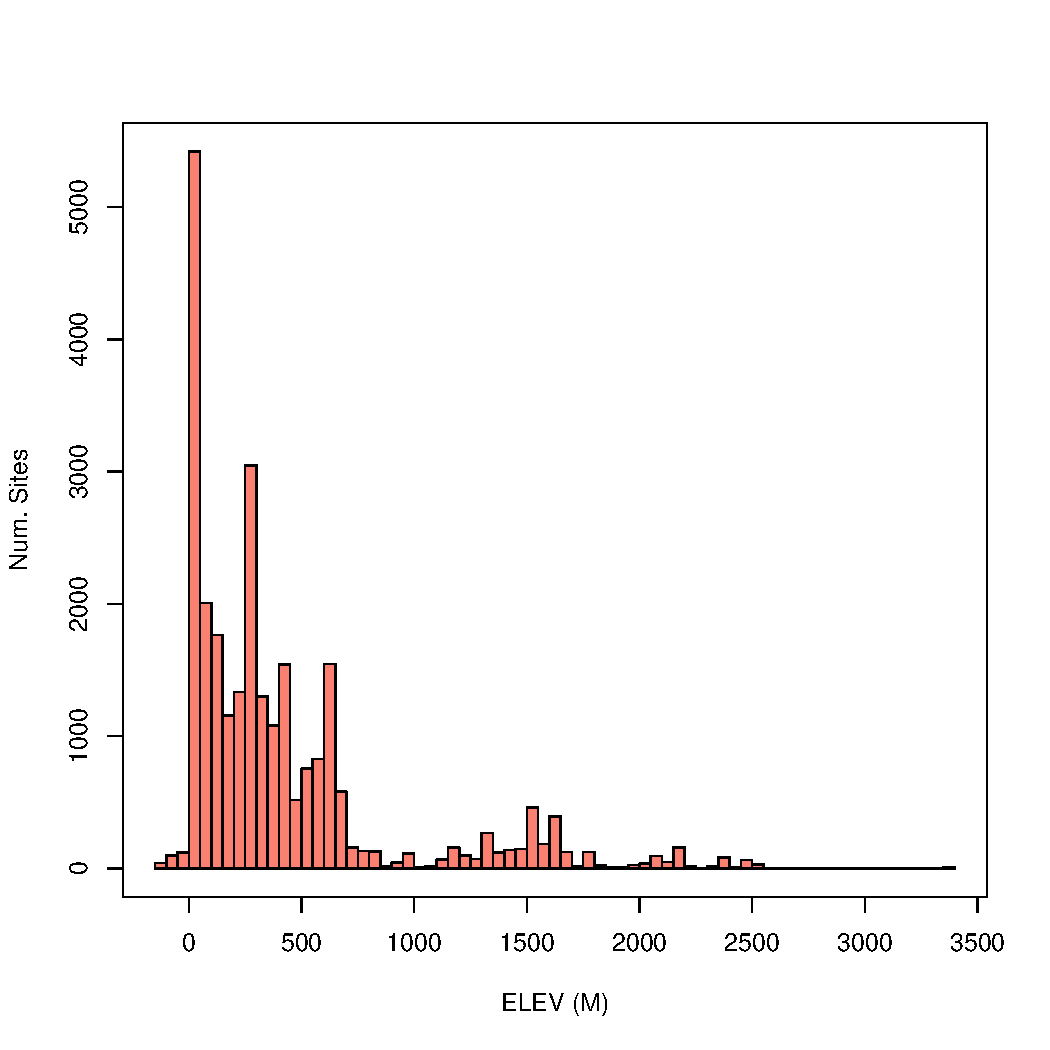
\includegraphics[width=6in]{Elevation}
\end{center}


\newpage
\section{Visualizing Data on Geographical Maps}

The phenological data that we are studying is best visualized on a map since the study sites are scattered all over the US states.  The maps will give us a better idea of the patterns that statistical analysis alone will not.  Making maps in R is relatively straightforward.  But we can't rely entirely on the functionality included in the base R distribution.  \\

\subsection{R Packages}
R is constantly under development and new versions come out routinely.  However, the base R distribution is not the only thing you have access to.  Thousands of specialized additions to R exist in the form of a library (also called a package) are available.  Comprehensive R Archive Network (CRAN: \url{https://cran.r-project.org}) is a website that archives much of these extra libraries/packages for downloads.  This archive is mirrored by hundreds of other servers scattered across the world.  You can look up a list of packages currently available on CRAN on this web page: \url{https://cran.r-project.org/web/packages/}.\\


\subsection{Loading Packages}
For our mapping exercise, we will need to enable several of these packages.  For convenience we have already installed these packages in the Virtualbox image that you are working inside.  All you need to do is to load these packages into R's memory space as follows.  The package {\tt ggplot2} is a comprehensive graphics library with its own R grammar.  The rest of the packages provide mapping utilities.\\

\begin{tcolorbox}[breakable,boxrule=0.5pt,enhanced]
\begin{code}

> library(ggplot2)
> library(maps)
> library(mapdata)

\end{code}
\end{tcolorbox}
\vspace{2ex}
 
Loading packages often generates some status messages on screen.  These messages can be informative.  For example, if a newly loaded package contains a function that is incompatible with an existing function, R tries to resolve that conflict.  You may or may not receive such messages today.\\


\subsection{Plotting a Base Map Layer}
A fully configured geographical map with some data superimposed upon it consists of several layers.  The basic foundation of a map is the determination of geographical area you want to plot (country, state etc.).  For this exercise, let's assume you want to plot the area of entire contiguous United States.  Below, we will slowly build up the map layer by layer.\\

\begin{tcolorbox}[breakable,boxrule=0.5pt,enhanced]
\begin{code}

> usa <- map_data(`usa')
> states <- map_data(`state')
> usa_base <- ggplot(data=states) + 
	geom_polygon(aes(x=long, y=lat, fill=I(`white'), group=group), color=`gray') + 
	coord_fixed(1.3) + guides(fill=FALSE) 
> usa_base
\end{code}
\end{tcolorbox}
\vspace{2ex}

Notice that the third command above has been split into three lines.  How does R know that those three lines are together?  The {\tt +} symbol will R that the command has not yet ended and to look for remaining parts of the command on the next line.  Breaking the code into different lines does not only make your code more readable, it ensures that you do not make any mistakes when typing.  The {\tt +} symbol provides a natural break for the eye.  There is second operator which can also be used for the purposes of breaking code into multiple lines.  That operator is a {\bf comma} ({\tt ,}).  You will see examples of both in this tutorial.\\

\begin{center}
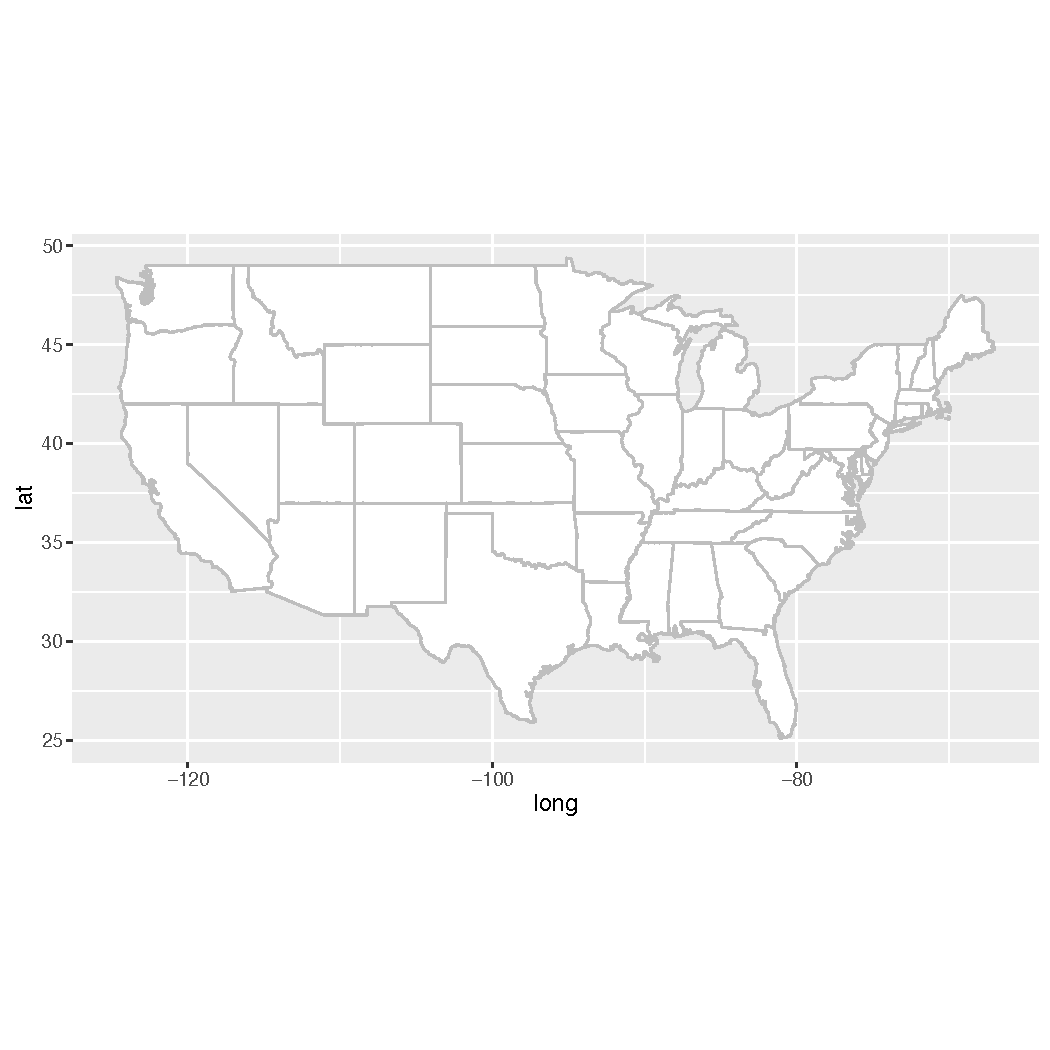
\includegraphics[width=6.5in]{usa_base}
\end{center}

\newpage
\subsection{Plot Points on the Map}
What good is a map if it doesn't show any data?  We will now plot the National Phenology Network's study sites onto the map.  We can do this using the geographical coordinates data (Longitude and Latitude) from the {\tt pheno} data set.  Notice how we created an R object called {\tt usa\_base} above.  This object now contains the base map layer we produced above.  So when we write more code to add points to this map, we would not have to repeat all of the code above.  Instead, we will just use the R object.\\


\begin{tcolorbox}[breakable,boxrule=0.5pt,enhanced]
\begin{code}

> usa_base + geom_point(data=pheno, aes(x=Longitude, y=Latitude), 
	color=`blue', cex=0.5, alpha=3/10) + 
	coord_fixed(xlim=c(-130,-60), ylim=c(25,50), ratio=1.3)
\end{code}
\end{tcolorbox}
\vspace{2ex}

\begin{center}
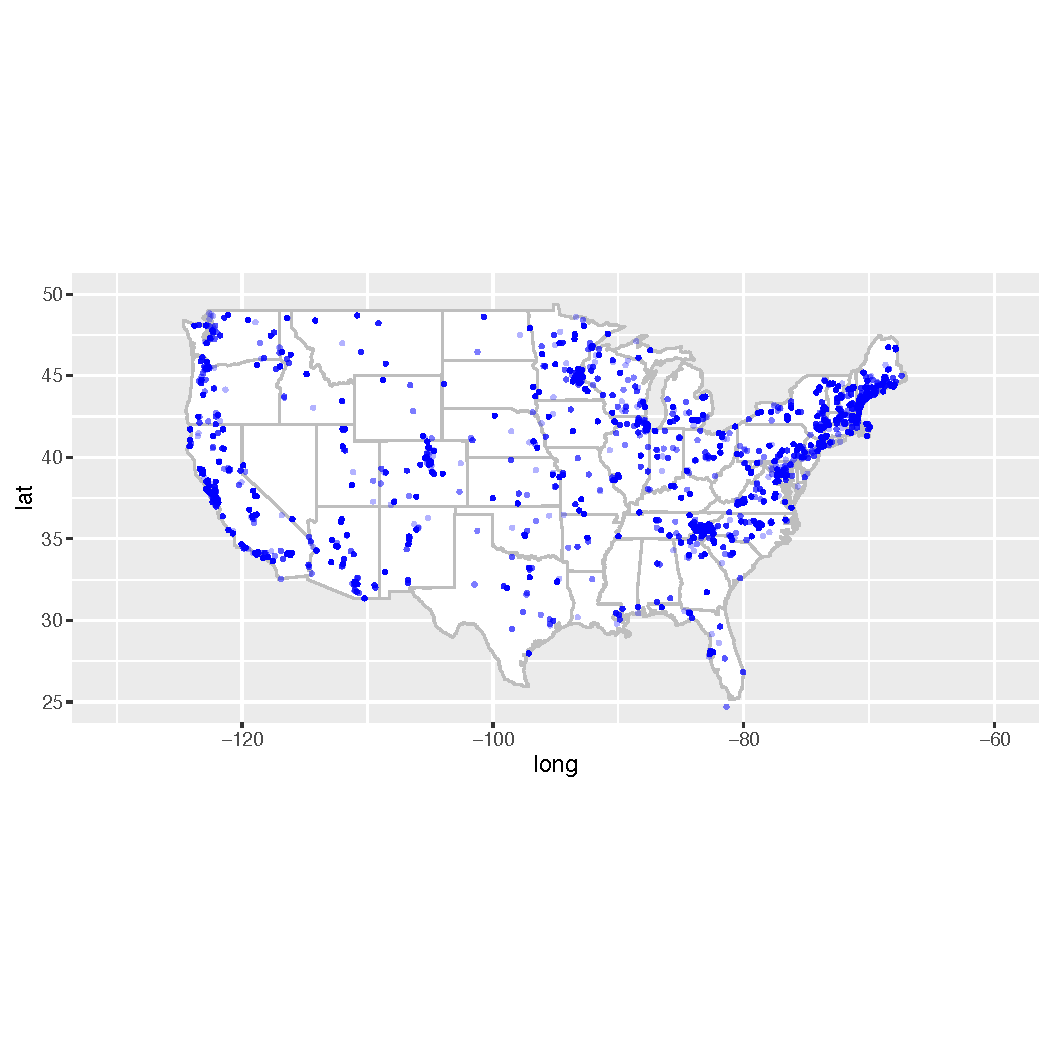
\includegraphics[width=6.5in]{usa_base_points}
\end{center}


\newpage
\subsection{Plot Elevation on the Map}
Want to make this plot even more interesting?  Let's adjust the point size by the amount of elevation at that site.  Try to notice the differences between the code above and below.\\


\begin{tcolorbox}[breakable,boxrule=0.5pt,enhanced]
\begin{code}

> usa_base + geom_point(data=pheno, aes(x=Longitude, y=Latitude), 
	color=`blue', cex=pheno$Elevation_in_Meters/1000, alpha=3/10) + 
	coord_fixed(xlim=c(-130,-60), ylim=c(25,50), ratio=1.3)
\end{code}
\end{tcolorbox}
\vspace{2ex}

\begin{center}
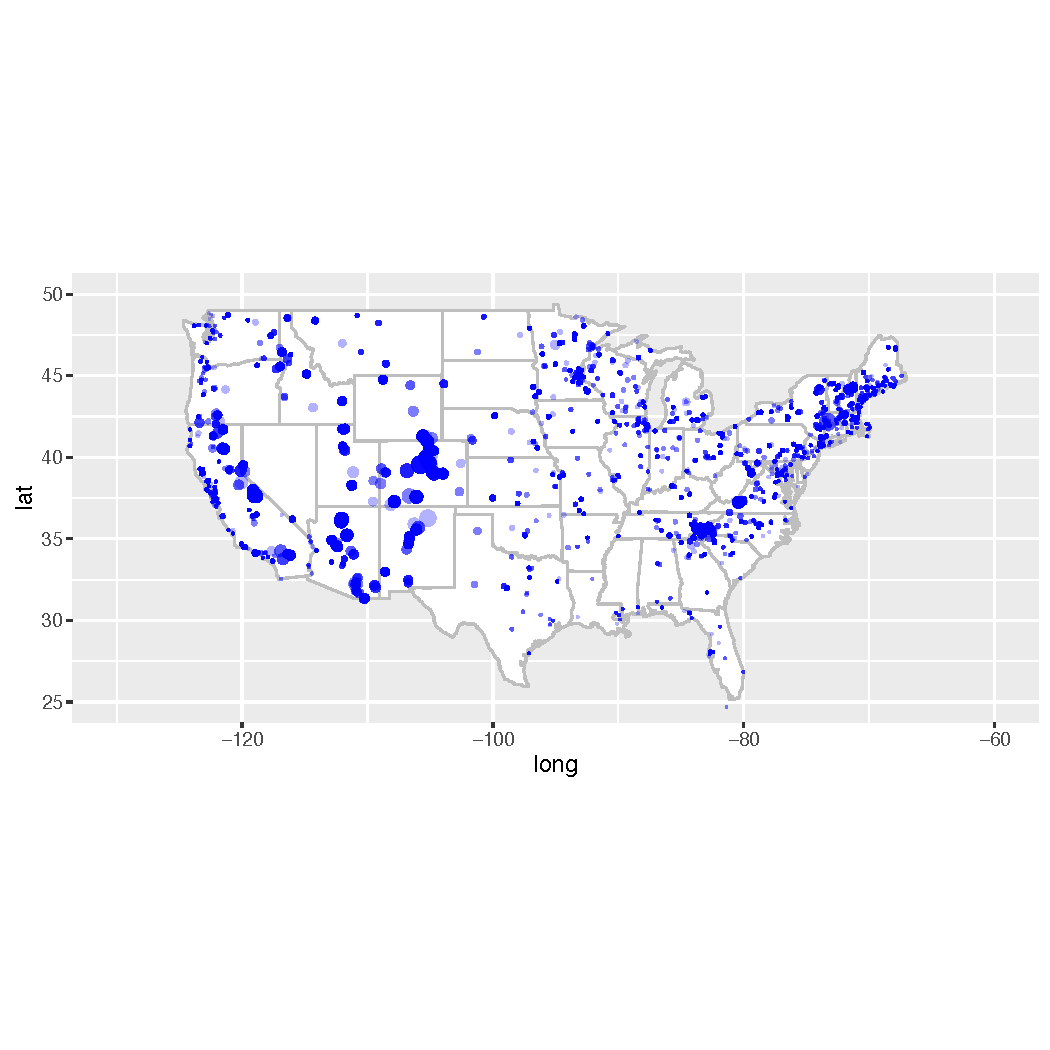
\includegraphics[width=6.5in]{usa_base_points_elevation}
\end{center}

Points that are larger indicate higher elevation than smaller ones.  Tiny points are almost at sea level or below.

\newpage
\section{Subsetting {\tt pheno} Dataset}
In order to visually determine whether the spring has been arriving early in recent years compared to previously, we will need to subset the {\tt pheno} dataset for several parameters:\\


\subsection{Subset Criteria}
\begin{enumerate}
\item {\bf Year}: We will limit the data to three growth years: 2010, 2013, 2016
\item {\bf Phenophase}: Data on several phenophases is available, but we will focus on 'bud break' data only
\item {\bf DOY}: Some species can have two bud breaks in a year and other anomalously do so.  We will avoid all of these by limiting our data to day of year 1 through 200.
\end{enumerate} 


\subsection{Subsetting Code in R}
The following code subsets the complete dataset using three parameters identified above into three separate R objects: {\tt pheno2010}, {\tt pheno2013} and {\tt pheno2016}. \\

\begin{tcolorbox}[breakable,boxrule=0.5pt,enhanced]
\begin{code}

> pheno2010 <- subset(pheno, 
	Phenophase_Description == `Breaking leaf buds' & 
	Mean_First_Yes_Year == 2010 & Median_First_Yes_DOY <= 200) 

> pheno2013 <- subset(pheno, 
	Phenophase_Description == `Breaking leaf buds' & 
	Mean_First_Yes_Year == 2013 & Median_First_Yes_DOY <= 200)

> pheno2016 <- subset(pheno, 
	Phenophase_Description == `Breaking leaf buds' & 
	Mean_First_Yes_Year == 2016 & Median_First_Yes_DOY <= 200)

\end{code}
\end{tcolorbox}
\vspace{2ex}


\subsection{Verify Subsetting}
Make sure the subsetting was done correctly. First check for the year.\\

\begin{tcolorbox}[breakable,boxrule=0.5pt,enhanced]
\begin{code}

> range(pheno2010$Mean_First_Yes_Year)
[1] 2010 2010

> range(pheno2013$Mean_First_Yes_Year)
[1] 2013 2013

> range(pheno2016$Mean_First_Yes_Year)
[1] 2016 2016

\end{code}
\end{tcolorbox}
\vspace{2ex}

Then check for the correct phenophase.  Here you might see phenophases other than `Breaking leaf buds', but their occurrences should be {\bf 0}.\\

\begin{tcolorbox}[breakable,boxrule=0.5pt,enhanced]
\begin{code}

> table(pheno2010$Phenophase_Description)
                          Breaking leaf buds 
                                         251 

> table(pheno2013$Phenophase_Description)
                          Breaking leaf buds 
                                         620

> table(pheno2016$Phenophase_Description)
                          Breaking leaf buds 
                                         921 

\end{code}
\end{tcolorbox}
\vspace{2ex}

Finally, make sure you do not have data beyond day 200 of the year.\\

\begin{tcolorbox}[breakable,boxrule=0.5pt,enhanced]
\begin{code}

> range(pheno2010$Median_First_Yes_DOY)
[1]  12 196
 
> range(pheno2013$Median_First_Yes_DOY)
[1]   7 198

> range(pheno2016$Median_First_Yes_DOY)
[1]   7 199

\end{code}
\end{tcolorbox}
\vspace{2ex}

Now we are ready for plotting these data on the geographical maps.  Using the same trick we used for the Elevation data, we will tie the size of points (Phenology record site location) to the data.  Only this time, we will associate the DOY parameter with the point size.  Therefore, we will associate {\bf early arrival of spring (early bud breaks)} with {\bf smaller point sizes} and {\bf later arrival of spring (late bud break)} with larger point sizes.  \\

We already have some idea as to the differences between these years given the relative numbers of observations in each year.  Let's see how those appear on the map.\\

\newpage


\section{Map Phenology Data}

\subsection{Spring of Year 2010}

The code for these plots is similar to the elevation plot.  Try to figure out what is different here.\\


\begin{tcolorbox}[breakable,boxrule=0.5pt,enhanced]
\begin{code}

> usa_base + geom_point(data=pheno2010, aes(x=Longitude, y=Latitude), 
	color=`darkgreen', cex=pheno2010$Median_First_Yes_DOY/50, alpha=3/10) + 
	coord_fixed(xlim=c(-130,-60), ylim=c(25,50), ratio=1.3)
\end{code}
\end{tcolorbox}
\vspace{1ex}

\begin{center}
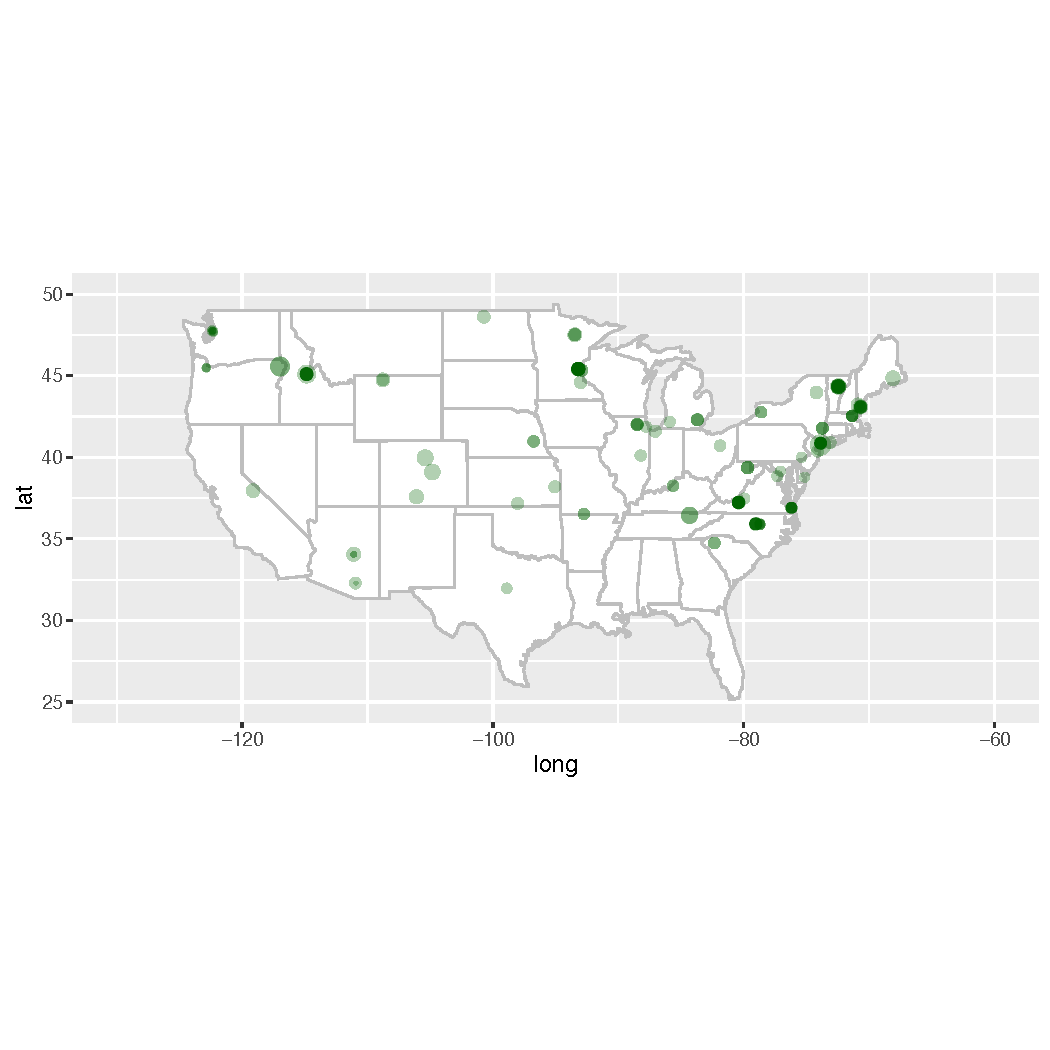
\includegraphics[width=6.5in]{pheno2010}
\end{center}

As you build maps for successive years, keep an eye out for how the landscape of phenology is changing over time.  Let the map for 2010 be your base threshold against which to compare spring in successive years.  There are two important questions that can be answered with these data: (1) Has spring been arriving sooner and sooner as time passes, and (2) Does this change happen within the same phenology observation site or new sites also pop up in successive years?


\subsection{Spring of Year 2013}

\begin{tcolorbox}[breakable,boxrule=0.5pt,enhanced]
\begin{code}

> usa_base + geom_point(data=pheno2013, aes(x=Longitude, y=Latitude), 
	color=`darkgreen', cex=pheno2013$Median_First_Yes_DOY/50, alpha=3/10) + 
	coord_fixed(xlim=c(-130,-60), ylim=c(25,50), ratio=1.3)
\end{code}
\end{tcolorbox}
\vspace{1ex}

\begin{center}
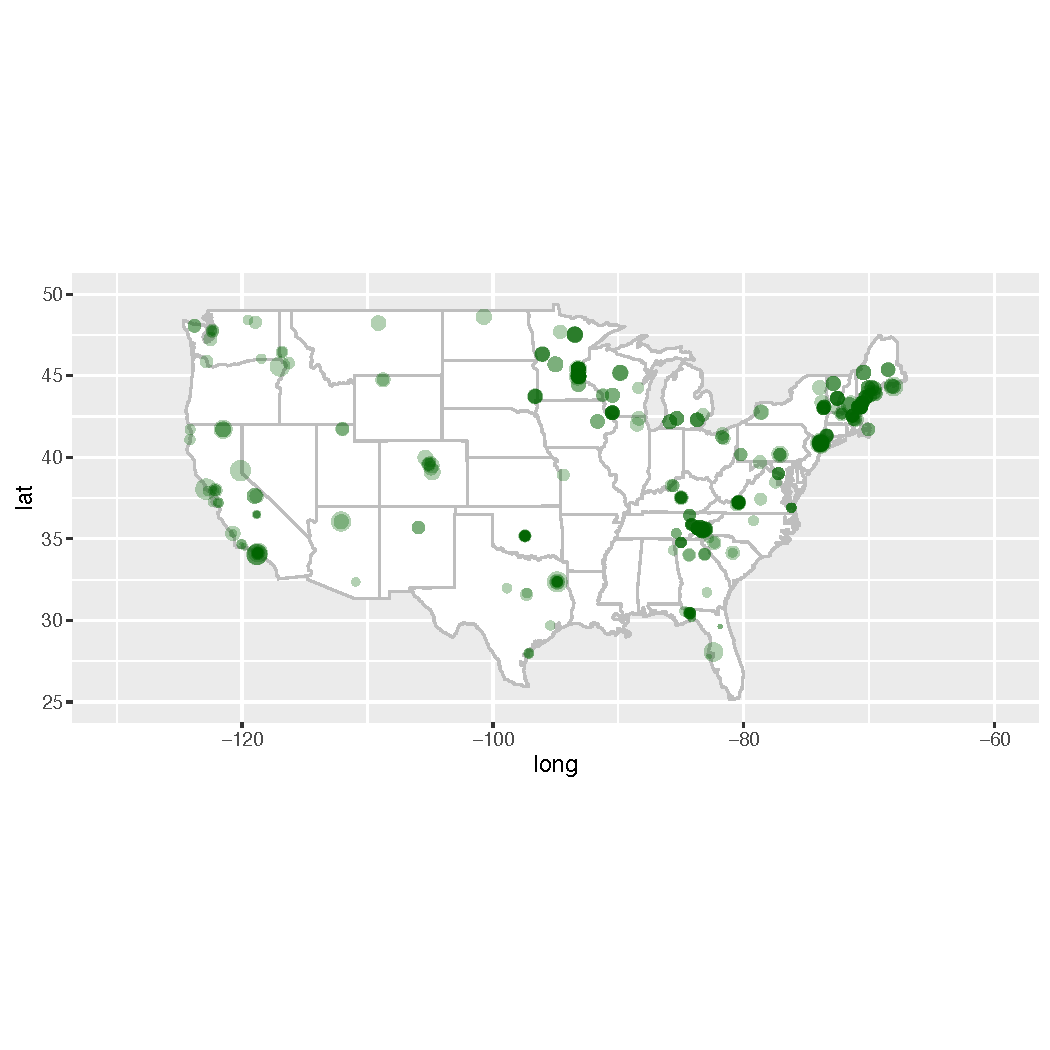
\includegraphics[width=6.5in]{pheno2013}
\end{center}



\subsection{Spring of Year 2016}

\begin{tcolorbox}[breakable,boxrule=0.5pt,enhanced]
\begin{code}

> usa_base + geom_point(data=pheno2016, aes(x=Longitude, y=Latitude), 
	color=`darkgreen', cex=pheno2016$Median_First_Yes_DOY/50, alpha=3/10) + 
	coord_fixed(xlim=c(-130,-60), ylim=c(25,50), ratio=1.3)
\end{code}
\end{tcolorbox}
\vspace{1ex}

\begin{center}
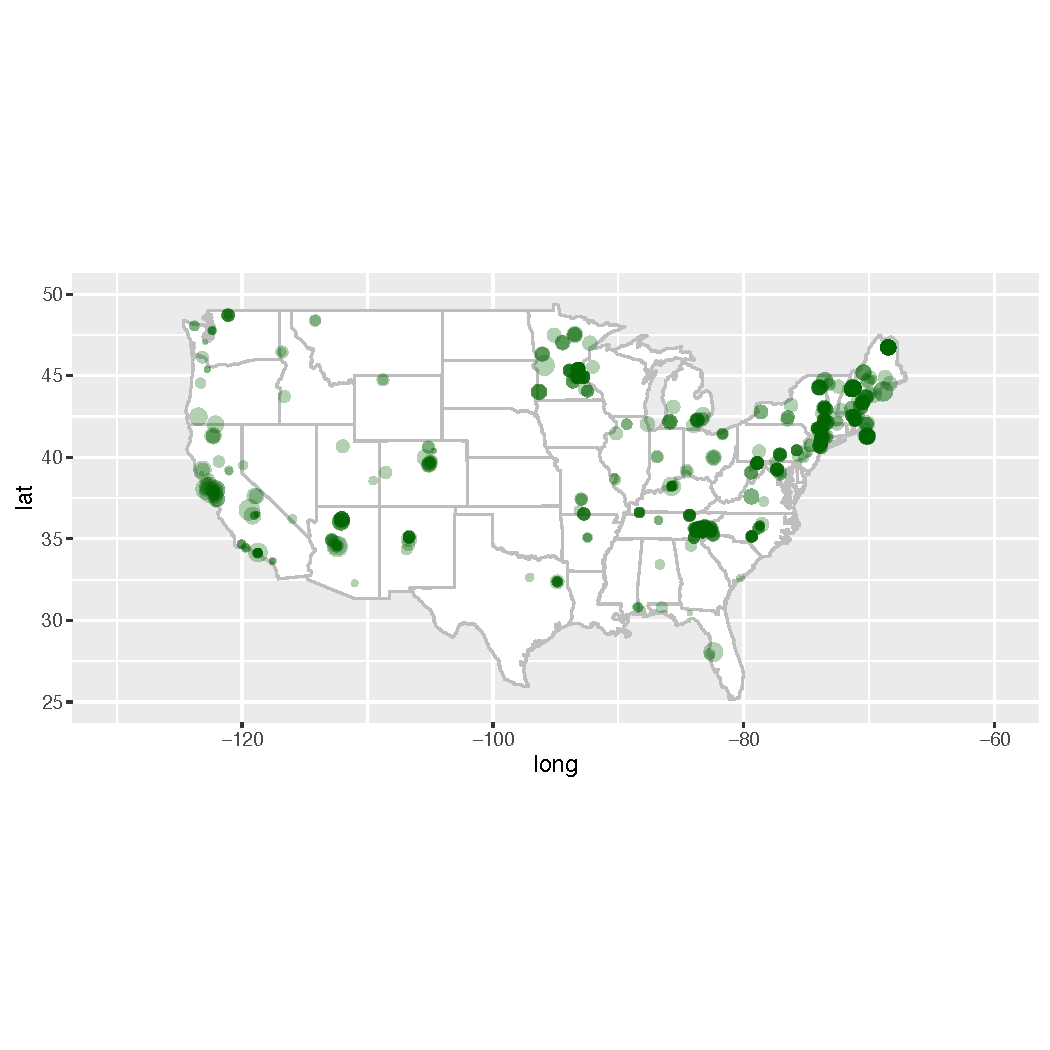
\includegraphics[width=6.5in]{pheno2016}
\end{center}

Based on your analysis of this data from the National Phenology Network across years 2010, 2013 and 2016, what is your inference about the onset of spring as it relates to phenology of plants?  






































































\end{document}


